\chapter{基础操作}
\label{cha:基础操作}

\section{机器人上电}

操作前,请再次确认已阅读并确保已遵循\prettyref{sec:安全指南}内容,排除潜在风险,确保操作安全。

\begin{figure}[hb]
    \centering
    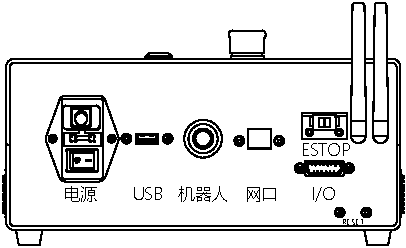
\includegraphics[height=4cm]{line_graphs/robot_control_box_back.pdf}
    \caption{控制箱背板示意图}
    \label{fig:控制箱背板示意图}
\end{figure}

\begin{enumerate}
\item 将机器人电缆插头插入控制箱的机器人接口;
\item 控制箱插上电源线,并将电源插头接入$220 \unit{V}$交流电插座;
\item 确保控制箱顶部的急停按钮处于释放\footnote{当机器按钮处于弹起状态时为释放状态,反之处于按下状态为锁定状态。}状态;
\item 打开控制箱背板的红色总电源开关,开关指示灯亮;
\item 长按控制箱顶部的开关机按钮或外接开关机按钮(选配)(约3 秒),直至控制箱顶部的开关机按钮的指示灯变成蓝色常亮,等待机器人肩部灯光亮起,完成控制箱和机器人的上电操作。
\end{enumerate}

\danger{\begin{itemize}
\item 请确保控制箱电源的插线板务必良好接地;
\item 请确保控制箱电源的输入电流受到漏电保护装置和适当的过流断路保护装置的保护;
\item 请确保所有的电缆在控制箱通电前都正确连接,始终正确使用原装的电源线。
\end{itemize}}

\danger[警告]{\begin{itemize}
\item 禁止在机器人启动时断开或用力拉拽机器人电缆;
\item 禁止延长或改动机器人电缆;
\item 切勿损坏电源线,或将重物压在电源线上;
\item 切勿使用破损或不符合的插座;
\item 切勿让电源插头和插座粘附灰尘和金属附着物。
\end{itemize}}

\clearpage

\section{连接机器人}
LM3支持有线网络连接和无线网络连接,无线网络连接目前仅支持接入控制箱内置的Wi-Fi热点网络。
\subsection{有线网络连接}

使用网线将控制箱背板的网口与路由器或交换机连接,同时确保用于操作机器人的电脑、平板、手机或其他图形化终端设备与机器人接入的是同一网络。

有线网络的连接示意如\prettyref{fig:有线网络连接拓扑图}:

\begin{figure}[ht]
    \centering
    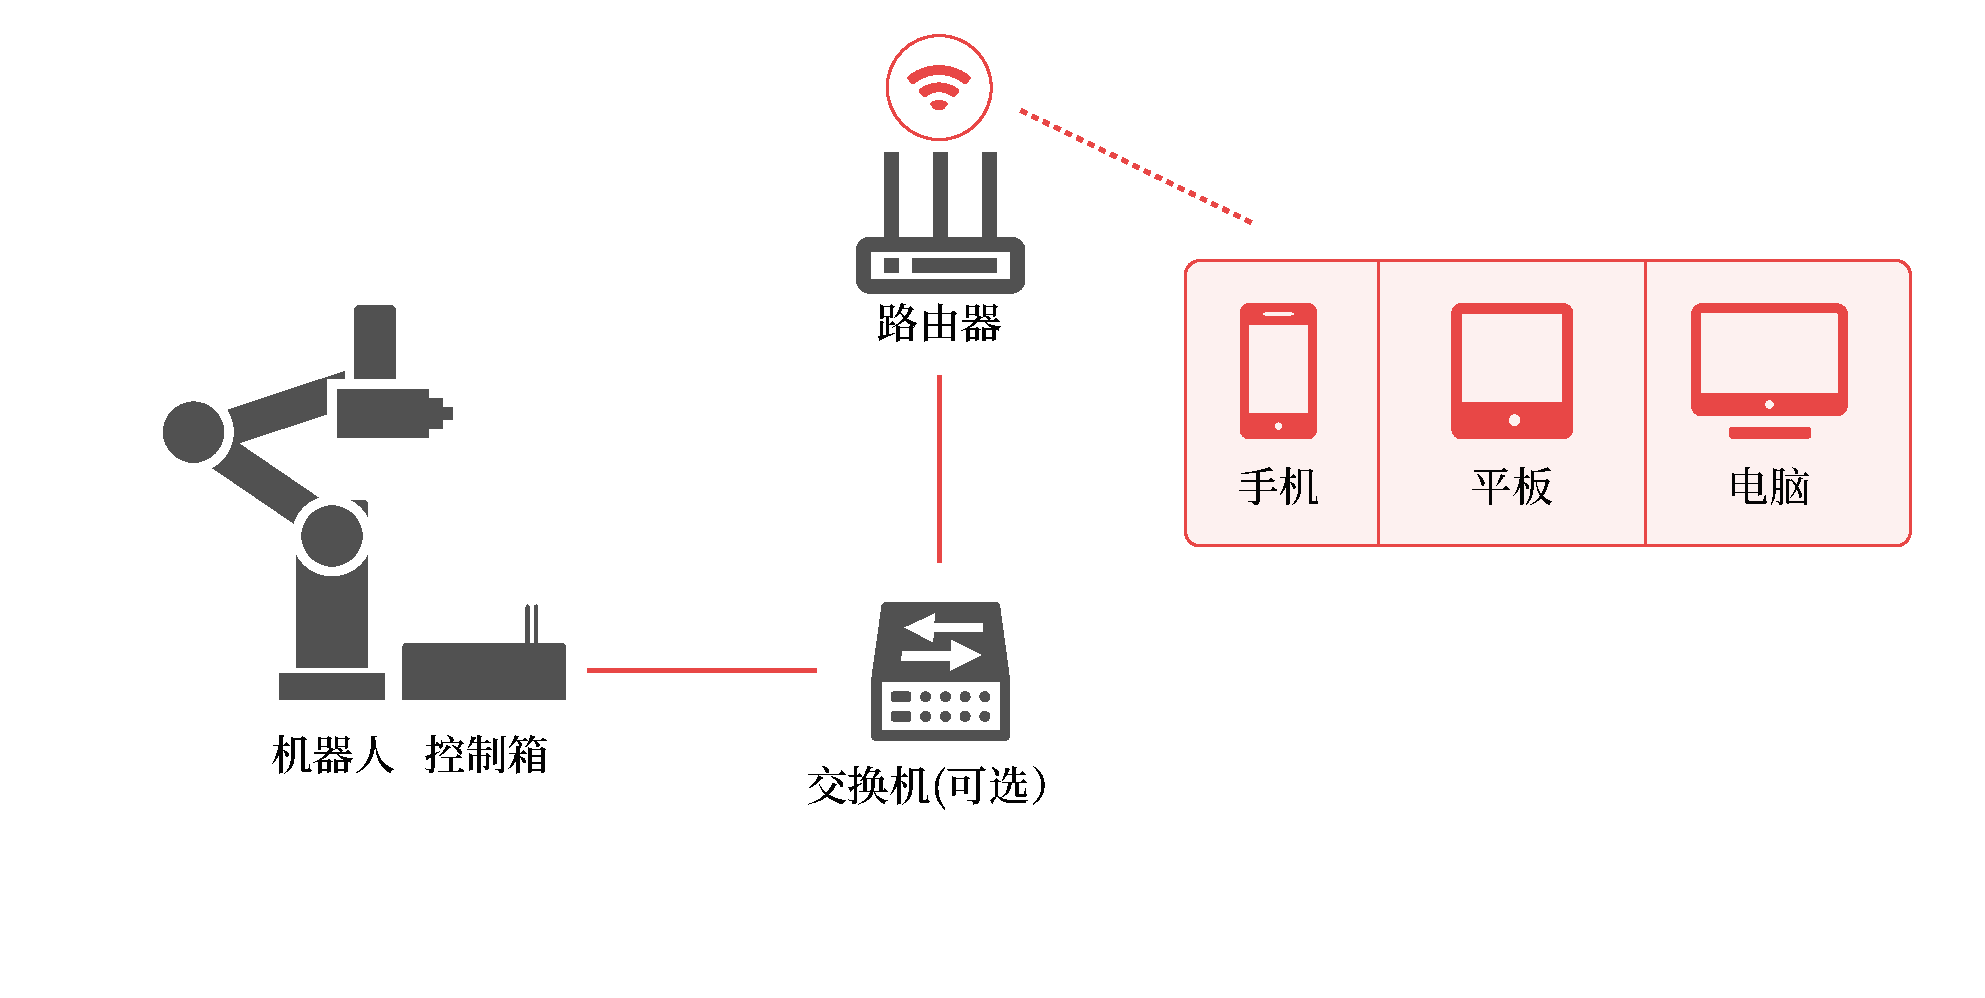
\includegraphics[width=\textwidth]{image/network-1.pdf}
    \caption{有线网络连接拓扑图}
    \label{fig:有线网络连接拓扑图}
\end{figure}

\clearpage

\subsection{无线网络连接}
机器人出厂后,默认会启用一个热点名称为设备名称\footnote{可在控制箱的铭牌上找到设备名称。}的Wi-Fi热点,设备名称格式如:\verb|Lebai-123456|(后6位为随机字符),默认密码为:\verb|88888888|(8个8)。可通过电脑、平板、手机或其他图形化终端设备的Wi-Fi功能连接该设备名称对应的Wi-Fi热点网络,连接和控制机器人。

\begin{figure}[ht]
    \centering
    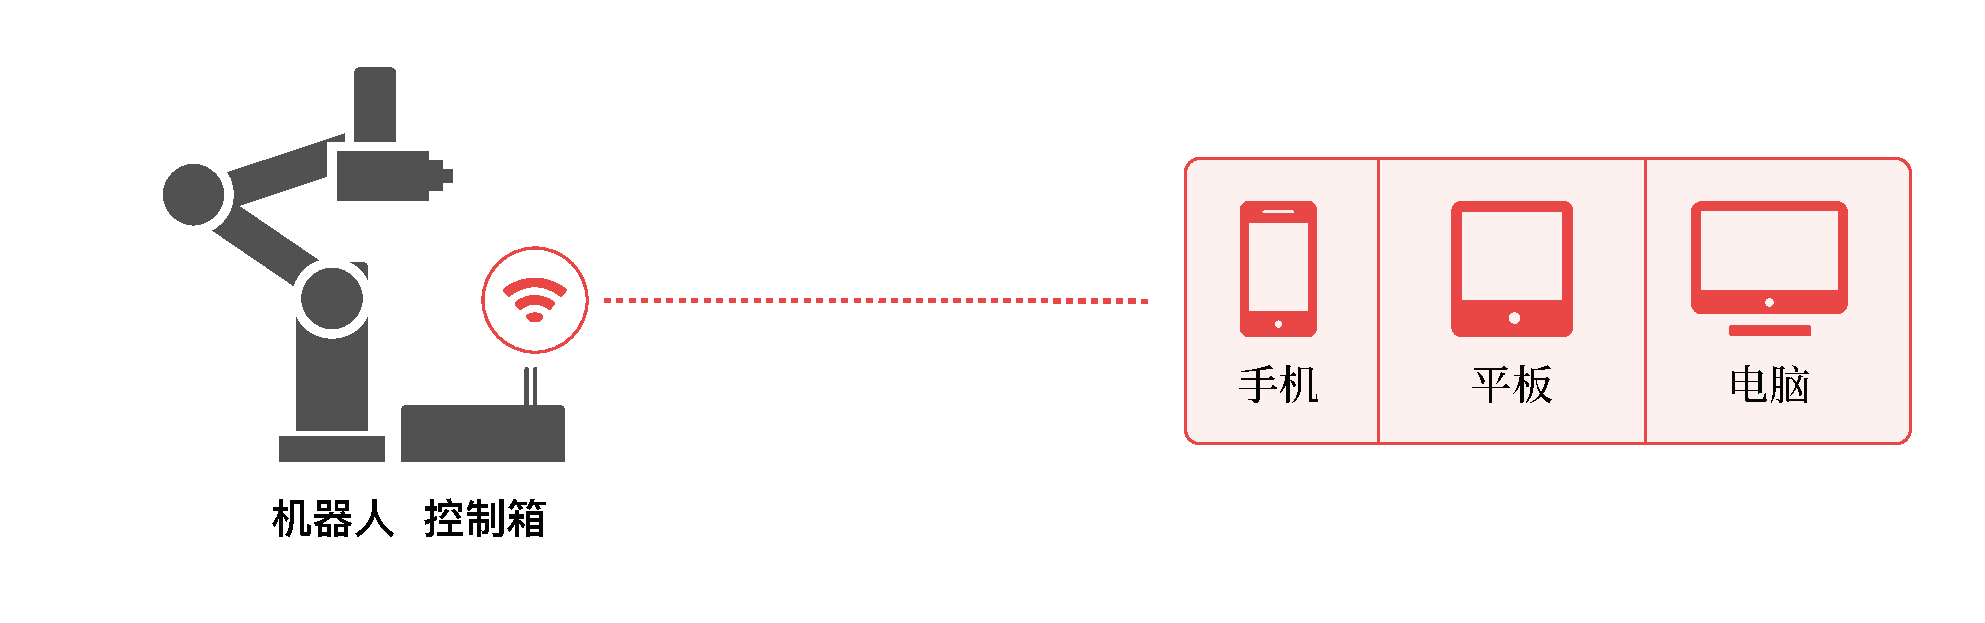
\includegraphics[width=\textwidth]{image/network-2.pdf}
    \caption{无线网络连接拓扑图}
    \label{fig:无线网络连接拓扑图}
\end{figure}

\clearpage

\section{登录\LM}
熟悉\LM 系统的操作将有助于您更方便和快速地上手使用本公司的机器人产品。
打开电脑、平板、手机或其他图形化终端设备的浏览器,在地址栏输入如下地址:
\begin{itemize}
	\item 若使用有线网络,地址为:\url{http://<IP>}\footnote{有线网络地址在接入的网络路由器页面中的设备列表里查看,查看方式因设备品牌和类型的不同而有差异,具体查看方式请参考路由器设备的说明书或联系对应设备厂商。}
	\item 若使用无线热点,地址为:\url{http://10.20.17.1}
\end{itemize}

网页打开后会进入登录页面,请输入默认授权码:\verb|1111|,点击\btn{登录}或按\kbd{Enter},登录\LM。

\begin{figure}[ht]
    \centering
    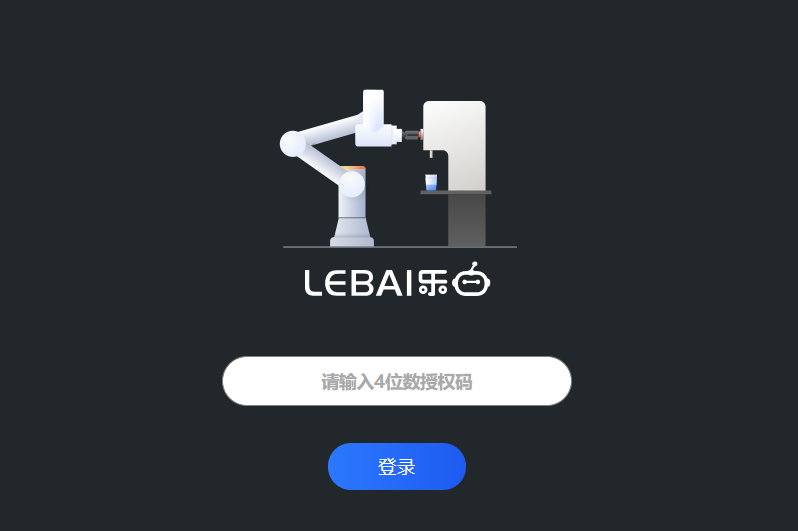
\includegraphics[width=0.8\textwidth]{screen/2-4.png}
    \caption{登录\LM}
    \label{fig:登录LM}
\end{figure}

\clearpage

\section{设置引导页}

当机器人开箱上电后,第一次登录\LM 时,首先需要按照设置引导页的提示进行初次使用的安装设置。
\subsection{系统设置}
第一步,在\mnu{系统设置}中可以自定义语言、时区、时间。

\begin{figure}[ht]
    \centering
    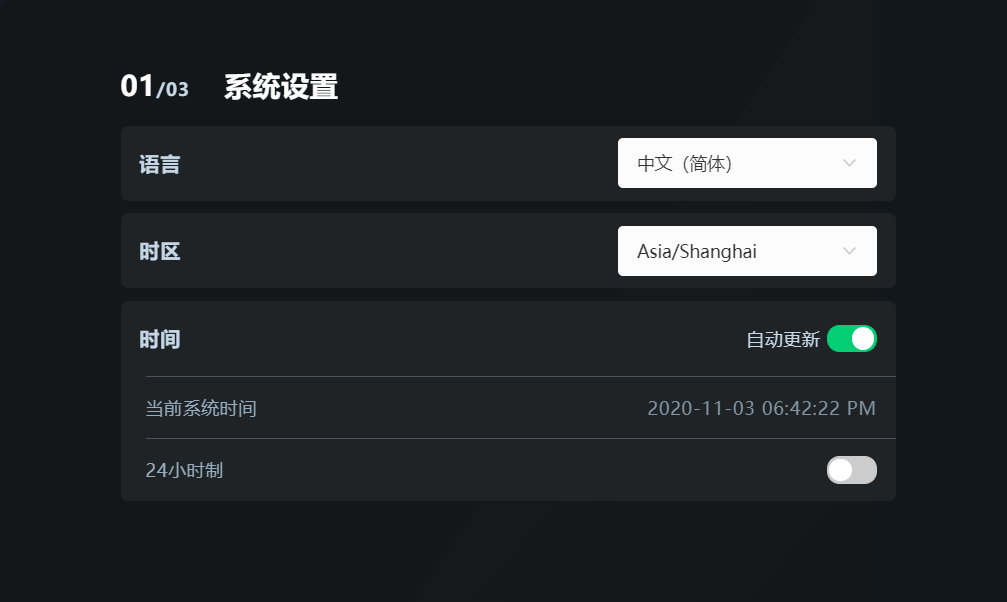
\includegraphics[width=\textwidth]{screen/2-5.png}
    \caption{系统设置}
    \label{fig:系统设置}
\end{figure}

\subsection{机器人设置}
第二步,在\mnu{机器人设置}中可以设置机器人的安装方式、操作模式及碰撞检测。
\begin{enumerate}
\item 安装方式

	根据实际安装方式,参照\prettyref{fig:安装方式}中的“图标对照表”选择正装、倒装、侧装。

	\begin{figure}[ht]
		\centering
		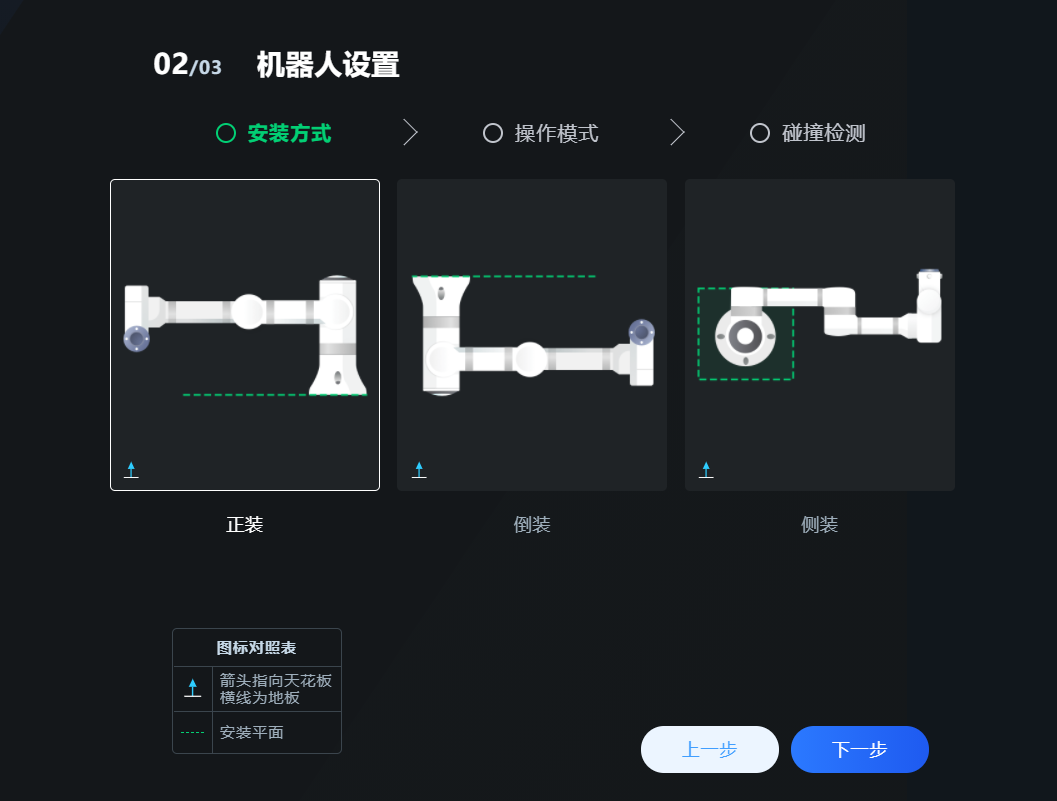
\includegraphics[width=\textwidth]{screen/2-6.png}
		\caption{安装方式}
		\label{fig:安装方式}
	\end{figure}

	\danger{安装方式的选择一定要与实际安装方式一致,否则有可能导致误伤。}

\clearpage

\item 操作模式

	可在\mnu{新手模式}和\mnu{专家模式}之间选择。\mnu{新手模式}适合没有编程基础的新手,无需理解任何逻辑和代码;\mnu{专家模式}适合有一定编程基础和逻辑基础的高级用户,您可以根据自身情况选择相应的操作模式。

	\begin{figure}[ht]
		\centering
		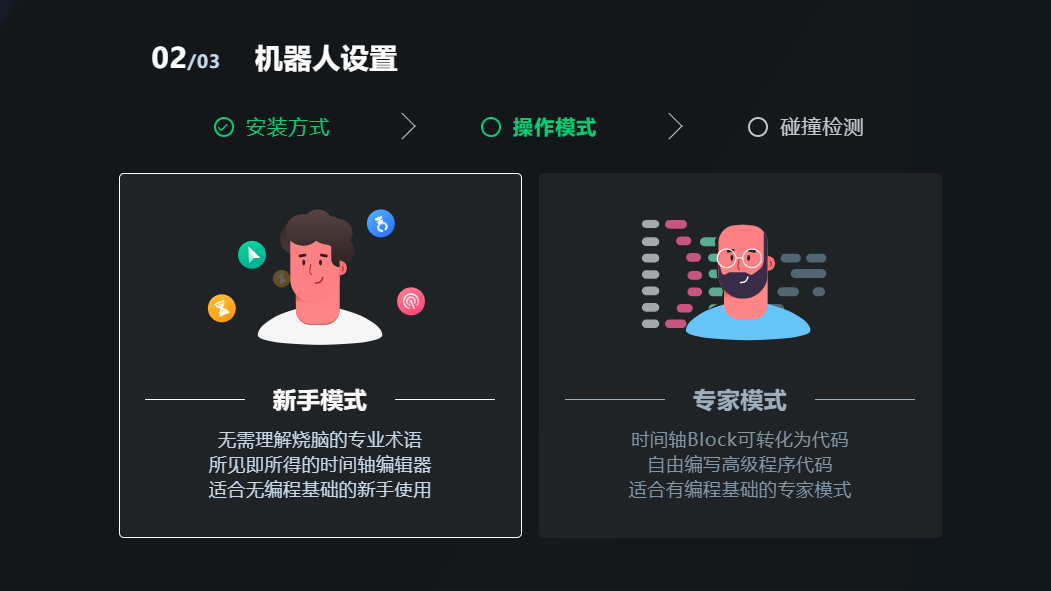
\includegraphics[width=\textwidth]{screen/2-7.png}
		\caption{操作模式}
		\label{fig:操作模式}
	\end{figure}

\clearpage

\item 碰撞检测

	检测开关默认为开,“碰撞后的动作”默认为\mnu{急停},可选择\mnu{急停}或\mnu{暂停},同时可以拖动拉杆来调整“检测灵敏度”大小。点击\btn{下一步},进入界面设置。

	\begin{figure}[ht]
		\centering
		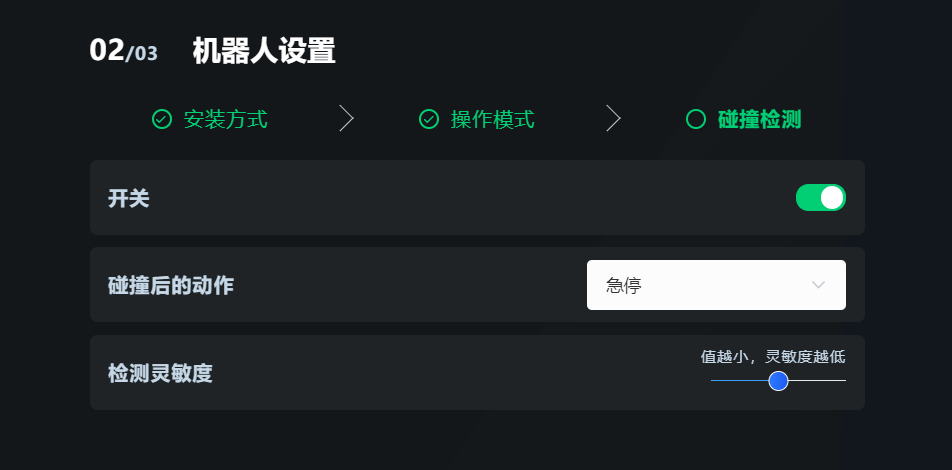
\includegraphics[width=\textwidth]{screen/2-8.png}
		\caption{碰撞检测}
		\label{fig:碰撞检测}
	\end{figure}

	\danger{机器人运行过程中,无论是否开启“碰撞检测”功能,禁止在没有防护的情况下进入到机器人作业半径范围内,否则存在人员被机器人撞伤的危险。}

\end{enumerate}

\clearpage

\subsection{界面设置}

第三步,在\mnu{界面设置}中,推荐使用\mnu{深色主题}。
% 可以选择\mnu{深色主题}或\mnu{浅色主题},目前\LM 浅色主题还在测试阶段,

\begin{figure}[ht]
	\centering
	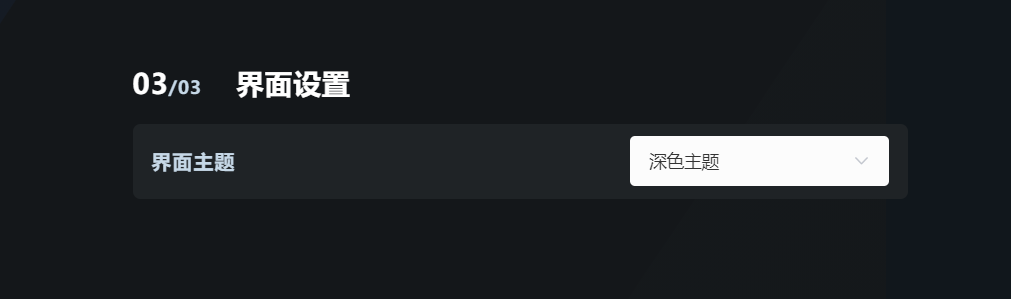
\includegraphics[width=\textwidth]{screen/2-9.png}
	\caption{界面设置}
	\label{fig:界面设置}
\end{figure}

点击\btn{完成},进入\LM 首页。

\clearpage

\section{首页}

在\LM 首页,页面分为:左面板、状态区、控制区、主功能入口、任务历史以及顶部标题栏六个区域。

\begin{itemize}
\item 左面板显示机器人整机温度及关节温度数据,坐标空间的位置和姿态数据,关节空间的关节角度数据;
\item 状态区显示机器人的实时状态;
\item 控制区包含机器人的启停按钮,软件示教按钮以及速度比例调整控件;
\item 主功能入口包含场景、控制和设备三个主功能入口;
\item 任务历史包含所有的任务历史列表;
\item 顶部标题栏右侧包含设置、消息中心和退出登录。
\end{itemize}

\begin{figure}[ht]
	\centering
	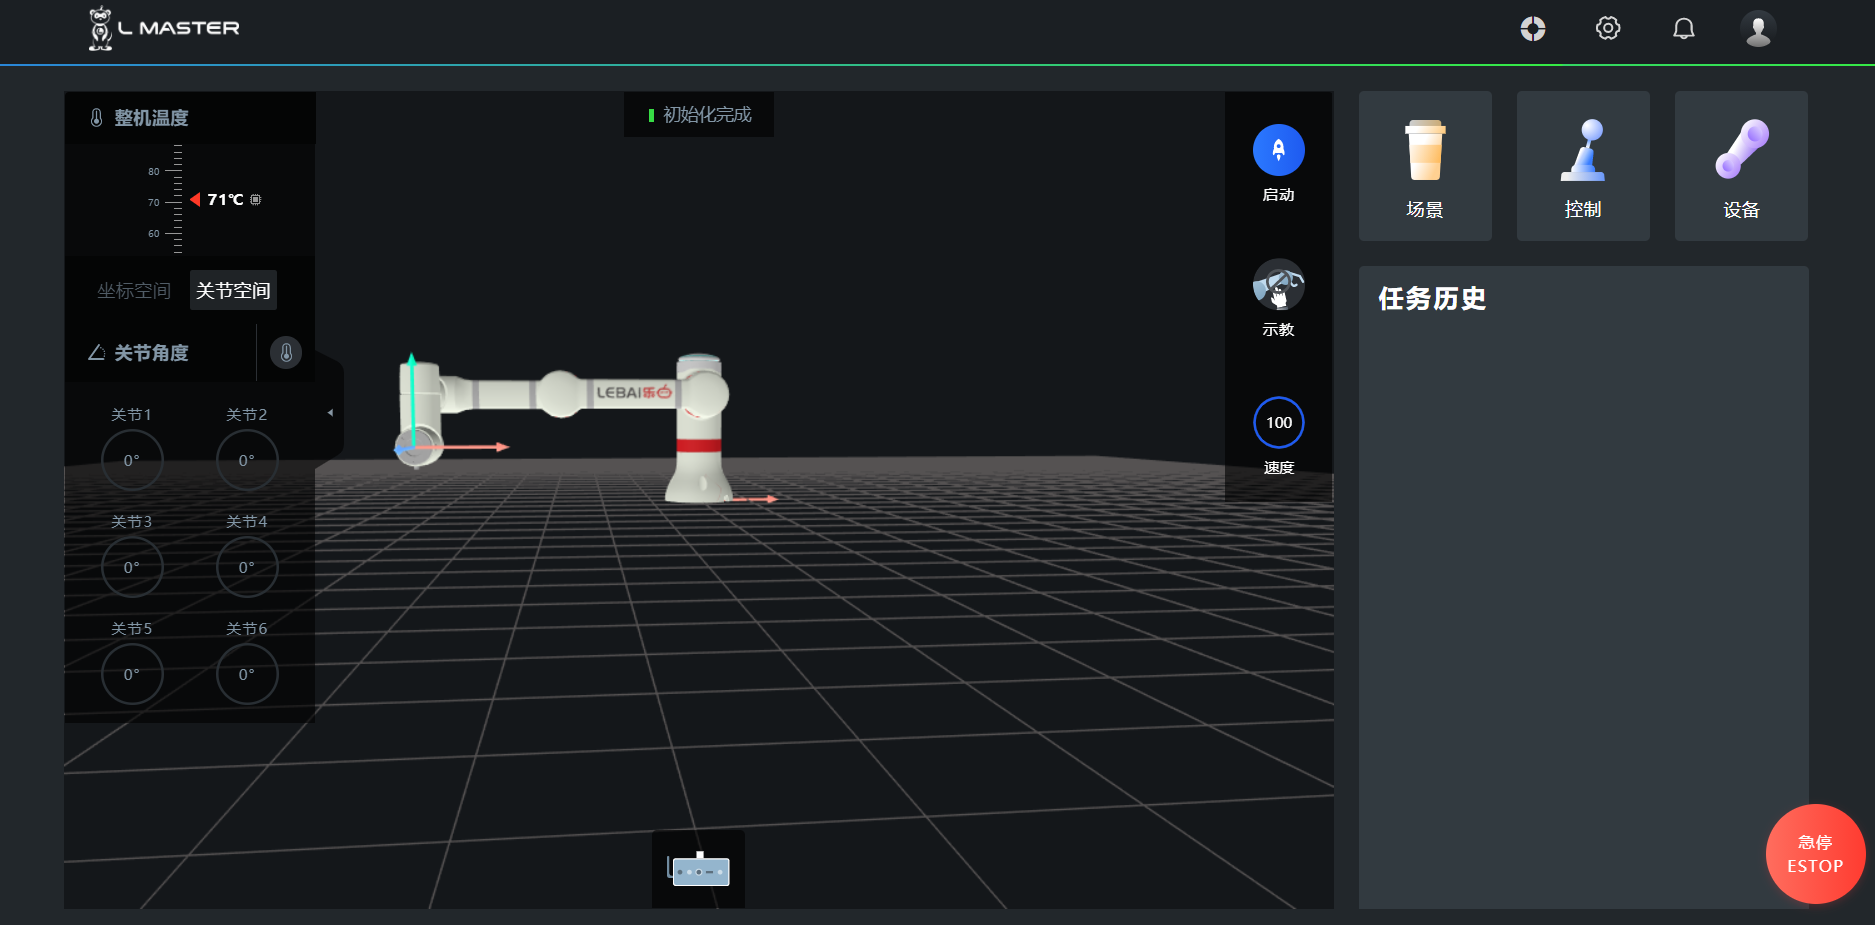
\includegraphics[width=\textwidth]{screen/2-10.png}
	\caption{\LM 首页}
	\label{fig:LM首页}
\end{figure}

\clearpage

\subsection{机器人状态}

机器人状态区显示机器人当前状态,具体说明可参考\prettyref{tab:机器人状态列表}。

\begin{table}[ht]
    \centering\small
	\rowcolors{1}{trEven}{trOdd}
    \begin{tabular}{ll}
\rowcolor{th}\Th{状态} & \Th{说明}\\
硬件通讯故障 & 机器人通讯故障或控制系统异常\\
已急停,请确认安全性 & 机器人处于急停状态\\
初始化中 & 机器人初始化中\\
初始化完成 & 机器人电源已开启\\
空闲 & 机器人处于空闲状态\\
运行中 & 机器人运行中\\
更新中 & 机器人系统更新中\\
启动中 & 机器人初始化完成到空闲的启动过程中\\
正在停止 & 机器人空闲状态转到停止状态\\
示教中 & 机器人处于示教模式中\\
已停止 & 机器人处于停止状态,非急停状态\\
    \end{tabular}
    \caption{机器人状态列表}
    \label{tab:机器人状态列表}
\end{table}

\vspace*{-3em}

\subsection{温度信息}
如\prettyref{fig:温度信息},\LM 首页左上方实时显示机器人的整机温度\footnote{取控制箱内控制器的CPU温度和机器人每个关节的温度的最大值作为整机温度的显示,当整机温度数值右侧显示芯片图标为表示当前CPU温度值最高,显示一个关节加数字图标时表示该数字对应的关节温度较高。},每个关节正常温度在室温至65 ℃之间。点击左面板\mnu{关节空间}右侧的~\icn{image/icon_temperature.pdf}~图标,可实时观测关节1至关节6的温度变化;再次点击该图标,可以切换回关节角度显示。

\vspace*{-1em}

\danger[警告]{当关节温度显示超过65℃时,请勿触摸机器人外表面,否则有高温烫伤风险,并请立即停机,待机器温度回到常温,再检查当前机器人负载是否超过额定有效负载$3\kg$或机器人是否碰撞到外部物品。}

\begin{figure}[ht]
	\centering
	\begin{minipage}[t]{0.32\linewidth}
		\centering
		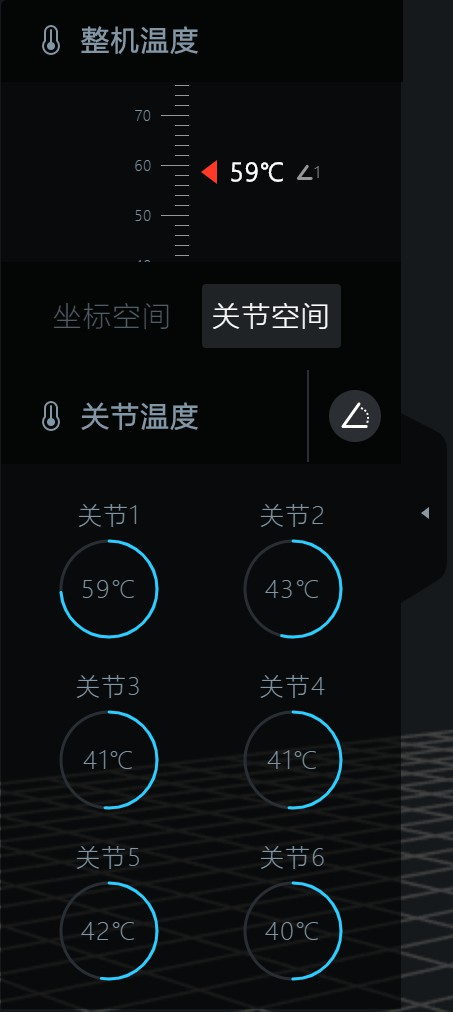
\includegraphics[height=6cm]{screen/2-11-t.jpg}
		\caption{关节温度}
		\label{fig:温度信息}
	\end{minipage}
	\begin{minipage}[t]{0.32\linewidth}
		\centering
		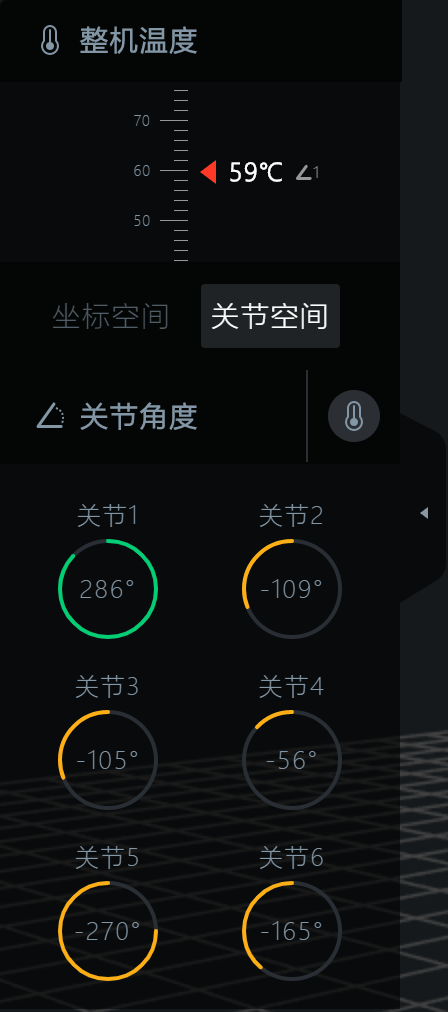
\includegraphics[height=6cm]{screen/2-12-1.png}
		\caption{关节空间}
		\label{fig:关节位置信息}
	\end{minipage}
	\begin{minipage}[t]{0.32\linewidth}
		\centering
		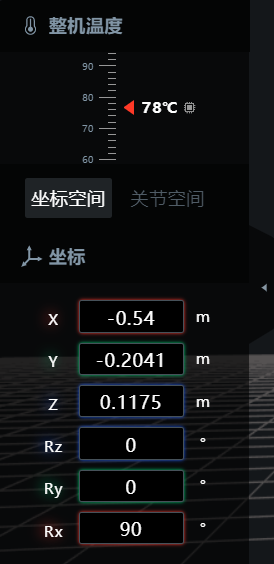
\includegraphics[height=6cm]{screen/2-12.png}
		\caption{坐标空间}
		\label{fig:坐标位置信息}
	\end{minipage}
\end{figure}

\vspace*{-2em}

\subsection{位置信息}
\LM 首页左面板实时同步机器人位置信息,包含坐标空间和关节空间。如\prettyref{fig:关节位置信息},关节空间显示机器人6个关节角度的实时数据;如\prettyref{fig:坐标位置信息},坐标空间显示机器人在坐标空间的位置和姿态的实时数据。

\subsection{速度比例}
点击\LM 首页控制区的速度图标,在展开的滑动条中拖动滑块或点击滑动条以调整机器人的运行速度比例,调整区间为$0\sim 100$。

\begin{figure}[ht]
	\centering
	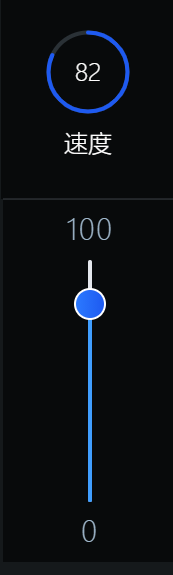
\includegraphics[height=4cm]{screen/2-13.png}
	\caption{速度比例}
	\label{fig:速度比例}
\end{figure}

\subsection{消息中心}
在消息中心中,可查看机器人提示、警告、软硬件异常的消息通知。鼠标移动到\LM 首页右上角的消息图标\colorbox{black}{\icn{image/22.pdf}}可以打开消息中心。

\begin{figure}[htb]
	\centering
	\begin{minipage}[t]{0.55\linewidth}
		\centering
		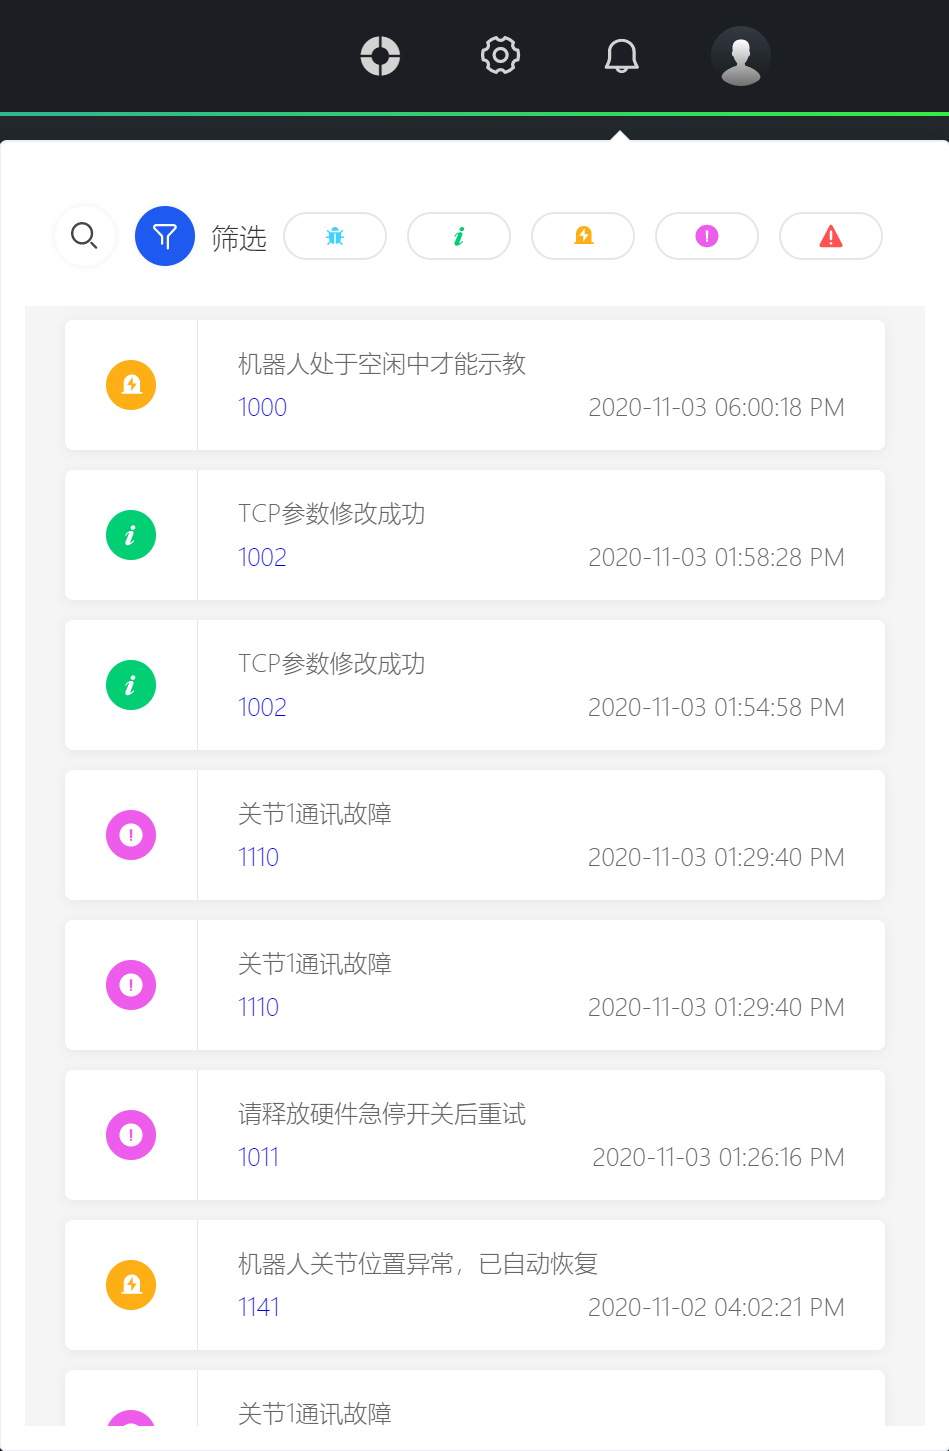
\includegraphics[height=8cm]{screen/2-14.png}
		\caption{消息中心}
		\label{fig:消息中心}
	\end{minipage}
	\hfill
	\begin{minipage}[t]{0.4\linewidth}
		\centering
		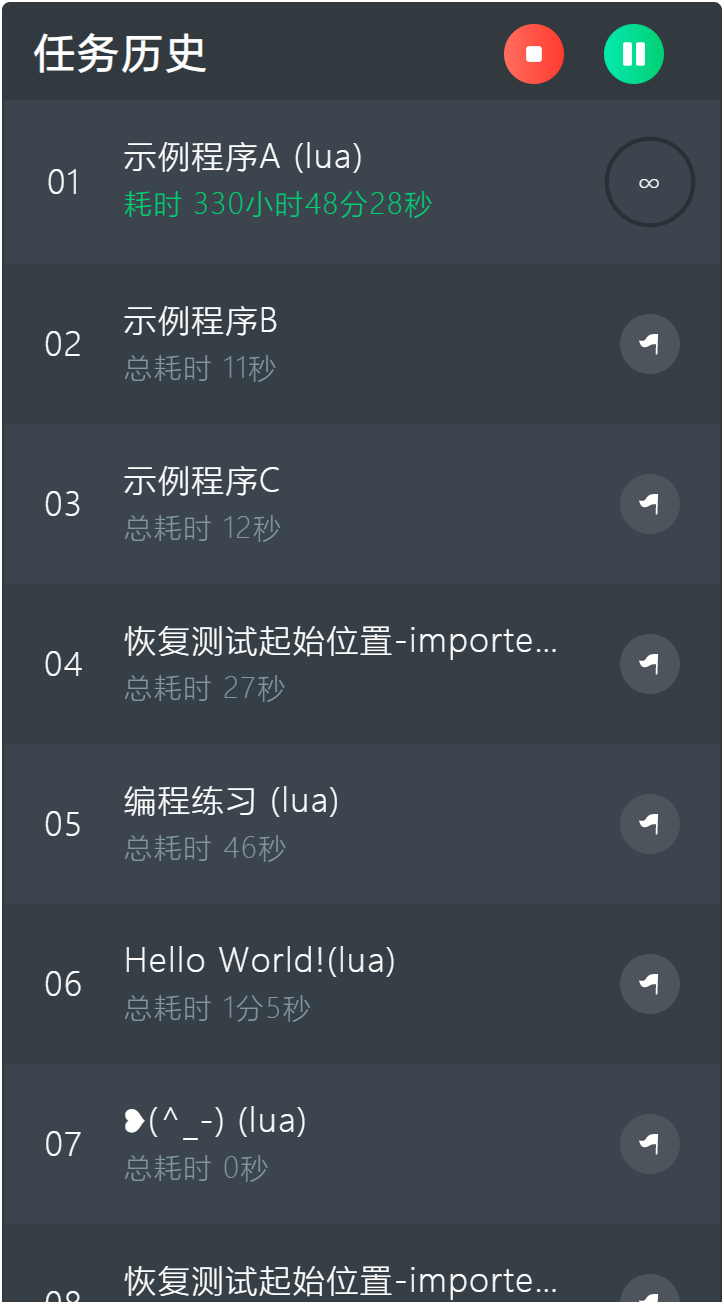
\includegraphics[height=8cm]{screen/2-15.png}
		\caption{任务历史}
		\label{fig:任务历史}
	\end{minipage}
\end{figure}
在消息中心中,有以下两种方式进行消息搜索:
\begin{enumerate}
	\item 通过关键字搜索消息通知;
	\item 通过筛选5种类型的机器人消息通知:
	\begin{itemize}
\item[\icn{image/30.pdf} 调试]
\item[\icn{image/29.pdf} 信息] 信息提醒类消息;
\item[\icn{image/28.pdf} 警告] 系统运行时警告级别的提醒,一般不影响使用;
\item[\icn{image/27.pdf} 错误] 系统出现了错误,需要保持关注错误的发生概率,如果频繁发生,需尽快点击查看解决方案或与本公司及时取得联系;
\item[\icn{image/26.pdf} 致命] 系统出现严重错误,存在运行风险或已无法正常运行,此时必须立即停机,查看解决方案或与本公司及时取得联系。
	\end{itemize}
\end{enumerate}

点击消息项的错误码超链接,可跳转至本公司官网对应的错误码解决方案页面,在页面中可根据错误码查找对应的问题及解决方案。

\subsection{任务历史}
\label{sec:任务历史}
任务历史列表中显示正在运行中及已完成的任务,并以时间顺序排列展现。当任务正在运行时,任务历史标题栏会出现停止、暂停或恢复的控制按键。任务历史列表中:
\begin{itemize}
	\item 正在运行的任务右侧显示当前已运行次数;
	\item 已完成的任务右侧显示\icn{image/icon_flag.pdf}~\mnu{重新运行}按钮,点击可重新运行当前选择的任务。
\end{itemize}

点击\mnu{任务历史}列表项任务名称,进入该任务对应的场景编辑页面。

\danger[警告]{当运行某个场景,该场景的任务进入任务历史列表。该任务运行完成,点击\mnu{重新运行}按钮后,当前执行的任务为之前执行该任务的场景数据,即使该场景在该任务运行完后发生变更,也不会影响该任务的重新运行,重新运行的任务不受该场景的数据变更影响,以上一次运行任务的场景数据为准。}

\clearpage

\section{启动机器人}
进入\LM ,如\prettyref{fig:启动机器人}所示,点击控制区的启动按钮;经过短暂的\mnu{启动中},首页状态区转为\mnu{空闲},表示您已成功启动机器人。

\begin{figure}[ht]
	\centering
	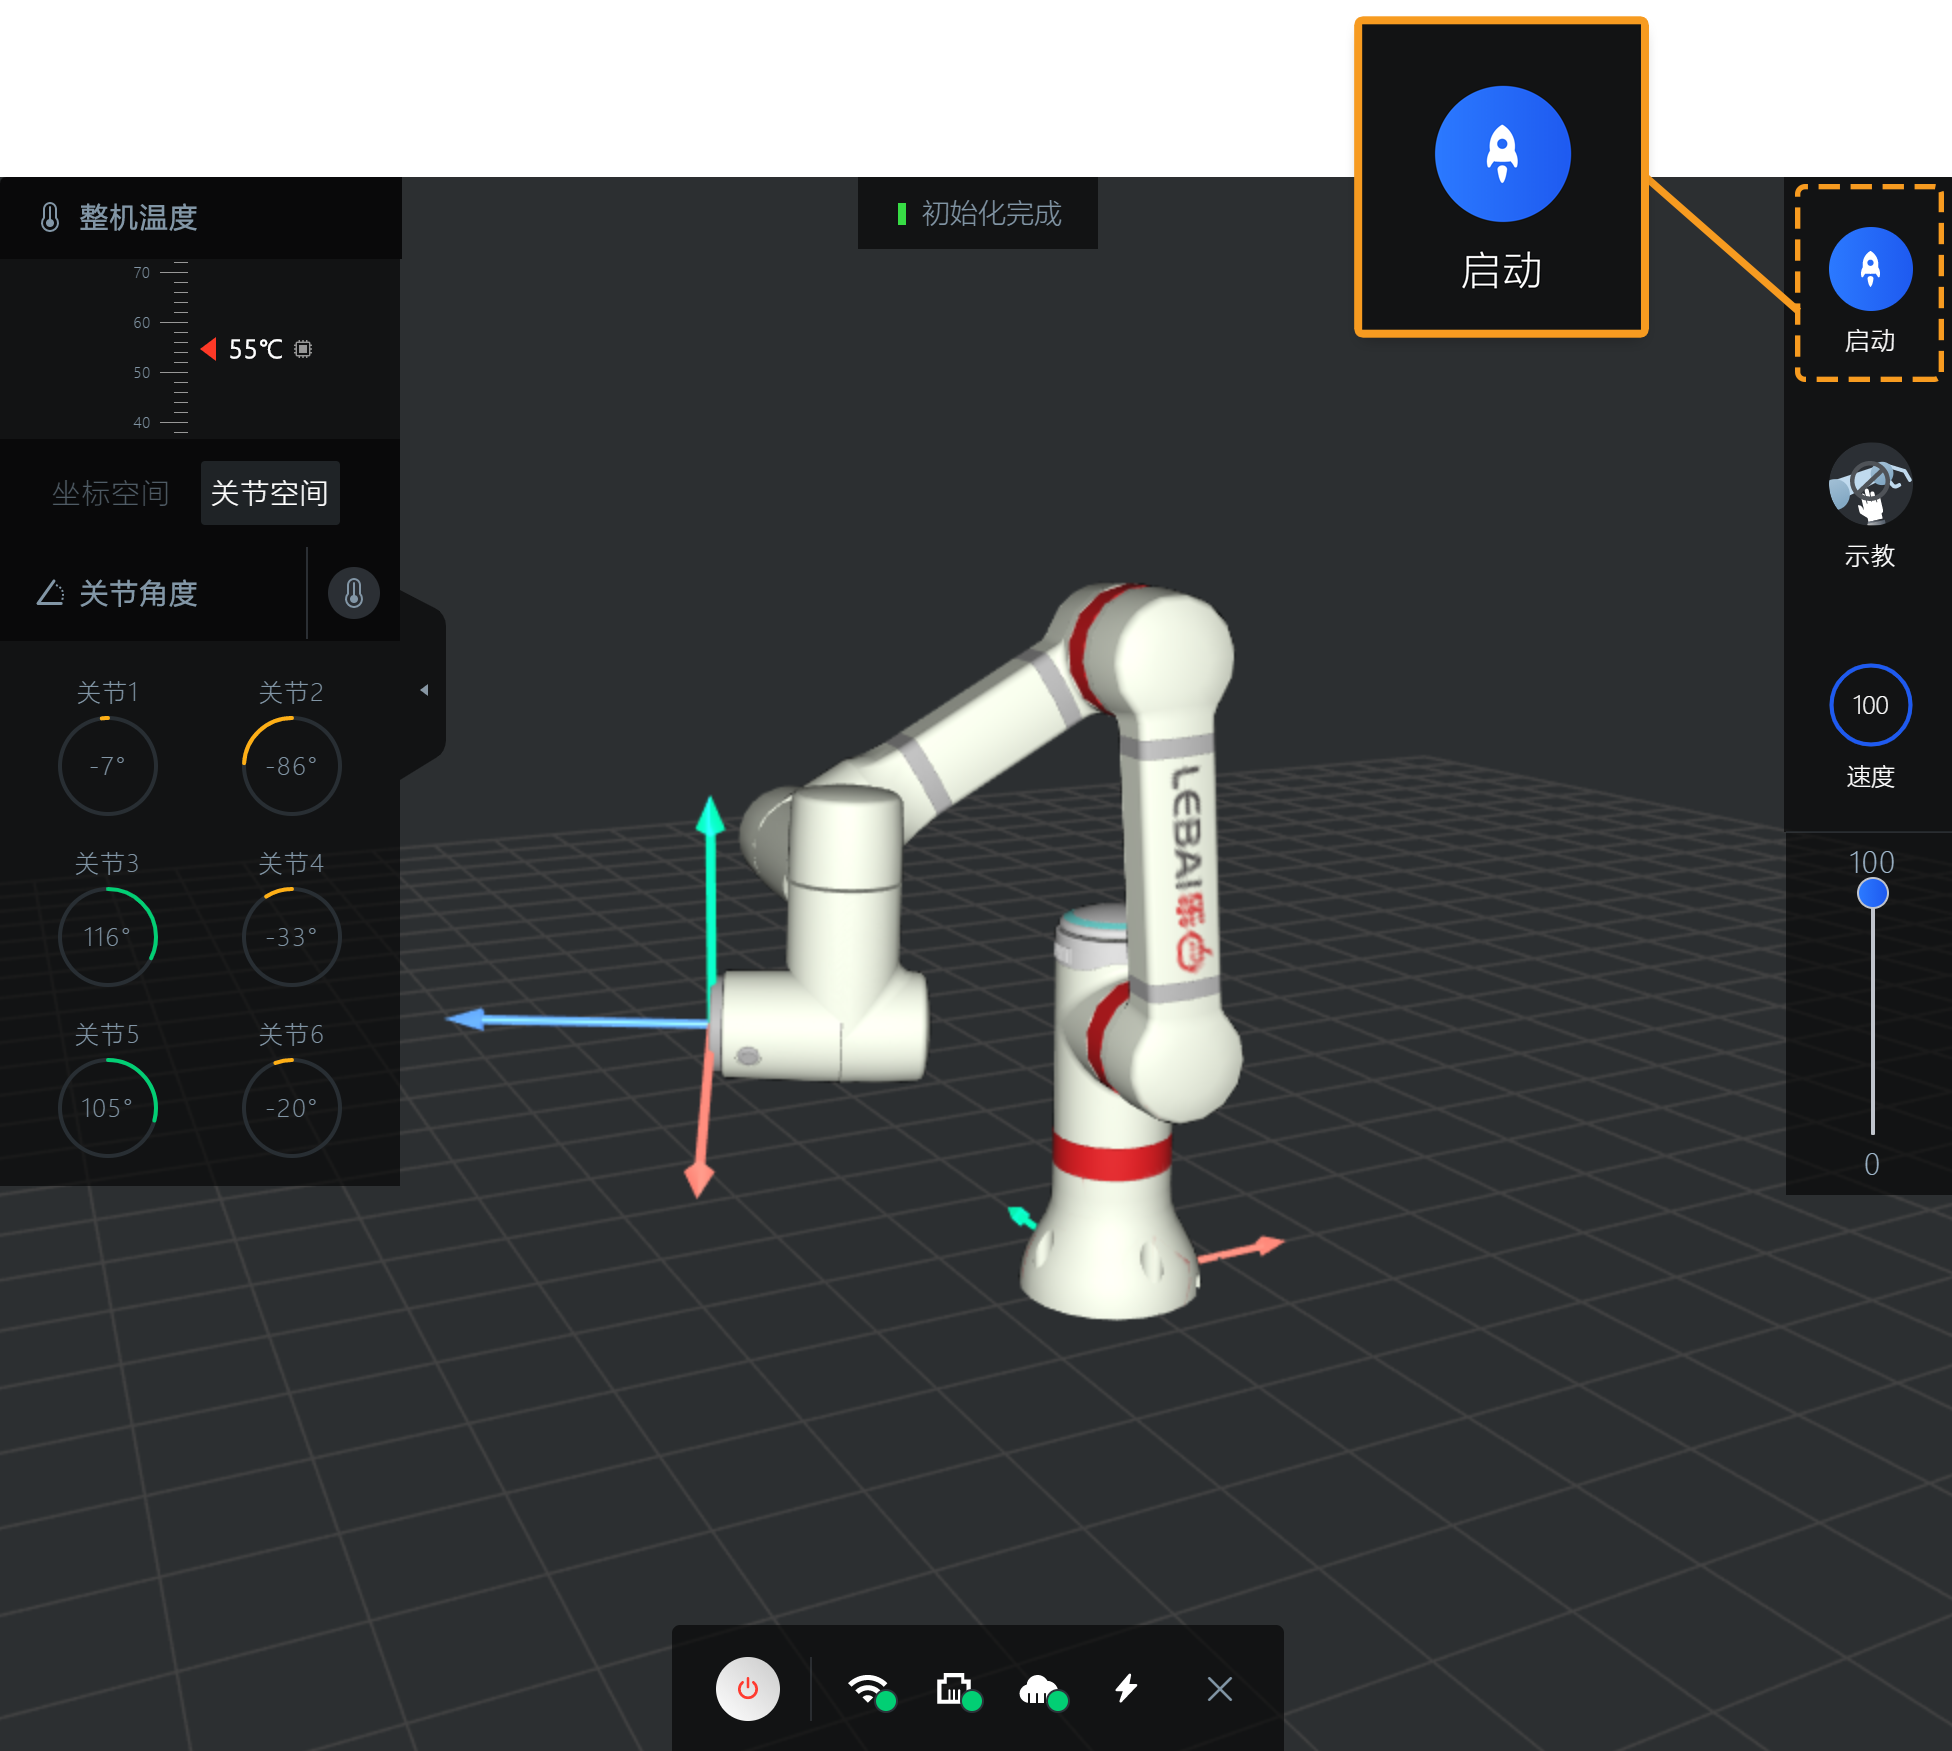
\includegraphics[width=\textwidth]{screen/2-16.png}
	\caption{启动机器人}
	\label{fig:启动机器人}
\end{figure}

\section{停止机器人}
当机器人处于\mnu{运行中}或\mnu{空闲}状态时,可以点击首页或如\prettyref{fig:胶囊控制区}所示的胶囊控制区的红色停止按钮;经过短暂的\mnu{停止中},当机器人状态变为\mnu{已停止}时,表示您已成功停止机器人。

% \begin{figure}[ht]
% 	\centering
% 	\includegraphics[width=\textwidth]{image/6.pdf}
% 	\caption{\LM  首页--停止机器人}
% 	\label{fig:停止机器人}
% \end{figure}

\section{急停机器人}

急停操作有两种方式,可任选其一:
\begin{itemize}[leftmargin=3.5em]
	\item[软急停] \LM 右下方的红色\btn[Danger]{急停ESTOP}按钮;
	\item[硬急停] 按下控制箱顶部的红色凸起急停按钮或外接急停按钮(选配)。
\end{itemize}

\info{使用硬急停操作后,急停操作不会自动释放,需要顺时针旋转急停按钮,解除锁定后完成释放。}

\section{关闭机器人}
\begin{enumerate}
	\item 先停止或者急停机器人;
	\item 长按控制箱开关机按钮或使用外置开关机按钮(选配),直至控制箱开关机按钮的蓝色指示灯熄灭;
	\item 关闭控制箱背板的红色总电源开关。
\end{enumerate}

\danger[警告]{关闭机器人需严格遵守上述操作步骤,否则可能导致机器人文件系统损坏、机器人功能故障等问题。}

\section{胶囊控制区}
胶囊控制区仅在非首页时显示,胶囊上半部分为\mnu{机器状态},胶囊下半部分为\mnu{任务历史}。长按胶囊本体可拖动调整胶囊控制区在页面中的位置。

\begin{figure}[hb]
	\centering
	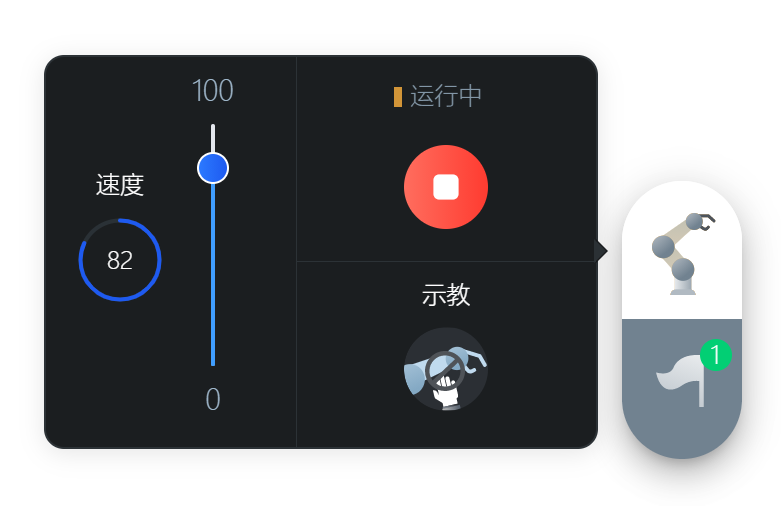
\includegraphics[height=4cm]{screen/2-18.png}
	\caption{胶囊控制区}
	\label{fig:胶囊控制区}
\end{figure}

\begin{itemize}[leftmargin=4.5em]
	\item [机器状态] 包含机器人当前状态、机器人启动/停止按钮、示教按钮以及速度调整拉杆,可以在非首页时操作和控制机器人;
	\item [任务历史] 包含正在运行中及已完成的任务列表、任务的暂停/恢复和停止按钮,可以在非首页时查看任务历史,具体操作见\prettyref{sec:任务历史}。
\end{itemize}
